\documentclass{beamer}

\mode<presentation>
{
   \usetheme{EEng}
%   \usetheme{Warsaw}
  \setbeamercovered{transparent}
  \setbeamercolor{background canvas}{bg=black!0}
}

\usepackage{enumerate}
\usepackage{array}
\usepackage{graphics}
\usepackage{ucs}
\usepackage[utf8x]{inputenc}
\usepackage[english]{babel}
\usepackage{amsmath, amsthm, amssymb}
\usepackage{amsmath}
\usepackage{amsfonts}
\usepackage{xcolor}
\usepackage{pgf}
\usepackage{hyperref}
\usepackage{url}
\usepackage{multicol}   % add-on
\usepackage{boxedminipage} 
\usepackage{indentfirst}   % add-on
\usepackage{float}
\usepackage[all]{xypic}
\usepackage{listings}
\usepackage{verbatim}
\usepackage{boxedminipage}

% % % inicio do listings e ref
\definecolor{darkblue}{rgb}{0,0,0.6}
\definecolor{gray_ulisses}{gray}{0.55}
\definecolor{castanho_ulisses}{rgb}{0.71,0.33,0.14}
\definecolor{preto_ulisses}{rgb}{0.41,0.20,0.04}
\definecolor{green_ulises}{rgb}{0.2,0.75,0}

\hypersetup{
    a4paper,
    pdftex,
    bookmarks,
    colorlinks,
    citecolor=darkblue,
    linkcolor=darkblue,
    urlcolor=darkblue,
    filecolor=darkblue
}

\lstdefinelanguage{perl_u} {
       basicstyle=\ttfamily\tiny,
       showstringspaces=false,
       breaklines=true,
       numbers=left,
       numberstyle=\tiny,
       numberblanklines=true,
       showspaces=false,
       showtabs=false
}
% % % fim do listings e ref

%\begin{figure}[htbp]
%\begin{center}
%
\includegraphics[width=0.9\textwidth]{images/DI-UM.PNG}
%\end{center}
%\end{figure}

\title{Stanford Parser e Tregex}
\author{José Pedro Silva \and
Pedro Faria \and
Ulisses Costa
}

\date{\today}
\institute{Engenharia de Linguagens\\
Processamento de Linguagem Natural
}

\AtBeginSubsection[] {
  \begin{frame}<beamer>
    \frametitle{Index}
    \scriptsize{\tableofcontents[currentsection,currentsubsection]}
  \end{frame}
}

\AtBeginSection[] {
  \begin{frame}<beamer>
    \frametitle{Index}
    \scriptsize{\tableofcontents[currentsection]}
  \end{frame}
}
\begin{document}
\begin{frame}
   \titlepage
\end{frame}

\section{Stanford}
\begin{frame} \frametitle{Stanford}
\begin{itemize}
 \item Software desenvolvido na Universidade de Stanford.
 \item Parser dedicado a extrair a estrutura gramatical de frases em linguagem natural.
 \item Entre as linguagens disponíveis temos: \begin{itemize}
                                               \item Inglês
					       \item Alemão
					       \item Mandarim
					       \item Árabe
                                              \end{itemize}
 \item Usado também para outras línguas (como o Português).
\end{itemize}

\end{frame}

\subsection{Interfaces}
\begin{frame} \frametitle{Interfaces}
 A aplicação, desenvolvida em \emph{Java}, tem disponível duas interfaces:
\begin{description}
 \item [Gráfica] usando tecnologia \emph{Java Swing}
 \item [Pelo terminal] através de \emph{scripts} escritos em \emph{csh}, uma linguagem \emph{bash} com \emph{syntax} equivalente a linguagem \texttt{C}
\end{description}
Optou-se por conduzir a exploração da ferramenta apenas pelo terminal.
\end{frame}

\subsection{Exemplos}
\begin{frame} \frametitle{Exemplo}
 Usou-se como caso de estudo o ficheiro \texttt{exem} com a frase:
 
\begin{block}{exem}
A simple complete sentence consists of a single clause.
\end{block}

Comando de execução

\begin{block}{comando}
./lexparser.csh exem
\end{block}

\end{frame}

\begin{frame}[fragile]\frametitle{Output 1}
O primeiro \emph{output} produzido é uma árvore com a estrutura gramatical da frase. Cada nodo da árvore está também decorado com
uma \emph{tag} correspondendo ao valor sintático da palavra:

\begin{lstlisting}[language=perl_u,breaklines=true]
 (ROOT
  (S
    (NP (DT A) (JJ simple) (JJ complete) (NN sentence))
    (VP (VBZ consists)
      (PP (IN of)
        (NP (DT a) (JJ single) (NN clause))))
    (. .)))
\end{lstlisting}

\end{frame}

\begin{frame}\frametitle{\emph{Tags}}
Lista de algumas definições de \emph{tags} do exemplo anterior.\\
 \begin{description}
  \item [S] - frase.
  \item [DT] - determinante.
  \item [JJ] - adjectivo ou numeral.
  \item [NN] - nome.
  \item [VBZ] - verbo no presente da 3ª pessoa do singular.
  \item [IN] - preposição ou conjunção.
 \end{description}
\end{frame}

\begin{frame}[fragile]\frametitle{Output 2}
 O segundo \emph{output} trata de apresentar relações gramaticais entre as palavras:
\begin{lstlisting}[language=perl_u,breaklines=true]
det(sentence-4, A-1)
amod(sentence-4, simple-2)
amod(sentence-4, complete-3)
nsubj(consists-5, sentence-4)
det(clause-9, a-7)
amod(clause-9, single-8)
prep\_of(consists-5, clause-9)
\end{lstlisting}

\end{frame}

\begin{frame}\frametitle{Exemplo de Relação}
  O seguinte output
 \begin{block}{}
  det(sentence-4, A-1)
 \end{block}
  representa a relação entre o determinante \texttt{'A'} com o nome \texttt{'sentence'}

\end{frame}

\section{Tregex}
\begin{frame}\frametitle{Tregex}
 A ferramenta \texttt{Tregex} é um utilitário para encontrar padrões em árvores produzidas pelo \texttt{Stanford Parser}.\\

 Através do primeiro \emph{output} da aplicação anterior, a aplicação produz uma árvore com \emph{highlight} nos padrões inseridos, neste caso a palavra \texttt{single}.  
\end{frame}

\begin{frame}\frametitle{Exemplo}
\begin{figure}[htbp]
\begin{center}
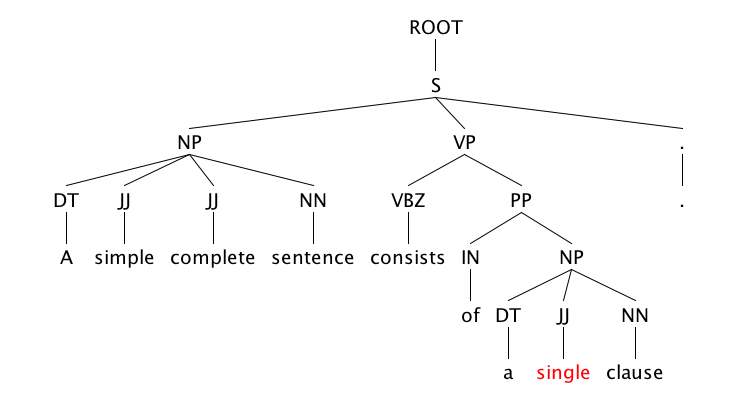
\includegraphics[width=0.9\textwidth]{images/scr.png}
\end{center}
\end{figure}

\end{frame}

\section{Tsurgeon}
\begin{frame}\frametitle{TSurgeon}
Tsurgeon é uma ferramenta que modifica árvores quando estas fazem \textit{match} de um determinado padrão. Sempre que a árvore corresponde ao padrão, é aplicada uma operação cirurgica à árvore.
\end{frame}

\begin{frame}\frametitle{Tipo de operações de transformação}
O Tsurgeon oferece uma vasta gama de transformações, desde a remoção de um nodo (e tudo o que depende dele), passando pela inserção de um nodo ou de uma árvore, até à movimentação de determinado nó na árvore.
\end{frame}

\subsection{Modo de utilização}
\begin{frame}\frametitle{Modo de utilização}
\begin{block}{}
./tsurgeon.csh -treeFile atree action
\end{block}
\begin{itemize}
\item atree : ficheiro que contém a árvore(s) que se pretende transformar
\item action : ficheiro que contém uma lista de padrões e uma lista de operações de transformação  
\end{itemize}
\end{frame}

\subsection{Exemplo}
\begin{frame}\frametitle{Exemplo}
\begin{block}{árvore a transformar}
(ROOT\\
  (S\\
    (NP (NNP Maria))\\
    (VP (VBD was)\\
      (VP (VBN arrested)\\
        (PP (IN in)\\
          (NP (NNP May)))))\\
    (. .)))\\
\end{block}
\end{frame}

\begin{frame}\frametitle{Exemplo}
\begin{block}{script de alteração}
VP \textless  PP = prep\\
delete prep
\end{block}
\begin{itemize}
\item \textbf{VP \textless  PP = prep} : esta expressão faz match a um nodo PP que seja filho directo de um nodo VP. O nodo PP é atribuido à variável \textit{prep}.
\item \textbf{delete prep} : comando que dita a eliminação do nodo prep
\end{itemize}
\end{frame}

\begin{frame}\frametitle{Exemplo}
\begin{block}{Resultado da transformação}
(ROOT\\
  (S\\
    (NP (NNP Maria))\\
    (VP (VBD was)\\
      (VP (VBN arrested)\\
    (. .)))\\
\end{block}
\begin{itemize}
\item o nodo PP foi eliminado, assim como os seus filhos.
\end{itemize}
\end{frame}


\section*{Perguntas}
\begin{frame} \frametitle{Perguntas}
\begin{center}\huge{?}\end{center}
\end{frame}

\end{document}

